
\chapter{Diccionarios}

\index{diccionarios} \index{diccionario} \index{tipo de datos!diccionario}
\index{clave} \index{par clave-valor} \index{índice}

Los tipos compuestos que ha visto hasta ahora (cadenas, listas y tuplas)
usan enteros como índices. Si usted intenta usar cualquier otro tipo
como índice provocará un error.

Los \textbf{diccionarios} son similares a otros tipos compuestos,
excepto en que pueden usar como índice cualquier tipo inmutable. A
modo de ejemplo, crearemos un diccionario que traduzca palabras inglesas
al español. En este diccionario, los índices son cadenas \texttt{(strings)}.

Una forma de crear un diccionario es empezar con el diccionario vacío
y añadir elementos. El diccionario vacío se expresa como \texttt{\{\}}:
\begin{verbatim}
>>> ing_a_esp = {}
>>> ing_a_esp['one'] = 'uno'
>>> ing_a_esp['two'] = 'dos'
\end{verbatim}

La primera asignación crea un diccionario llamado \texttt{ing\_a\_esp};
las otras asignaciones añaden nuevos elementos al diccionario. Podemos
desplegar el valor actual del diccionario del modo habitual:
\begin{verbatim}
>>> print(ing_a_esp)
{'one': 'uno', 'two': 'dos'}
\end{verbatim}

Los elementos de un diccionario aparecen en una lista separada por
comas. Cada entrada contiene un índice y un valor separado por dos
puntos (:). En un diccionario, los índices se llaman \textbf{claves},
por eso los elementos se llaman \textbf{pares clave-valor}.

Otra forma de crear un diccionario es dando una lista de pares clave-valor
con la misma sintaxis que la salida del ejemplo anterior:
\begin{verbatim}
>>> ing_a_esp={'one': 'uno', 'two': 'dos', 'three': 'tres'}
\end{verbatim}

Si volvemos a imprimir el valor de \texttt{ing\_a\_esp}, nos llevamos
una sorpresa:
\begin{verbatim}
>>> print(ing_a_esp)
{'one': 'uno', 'three': 'tres', 'two': 'dos'}
\end{verbatim}

¡Los pares clave-valor no están en orden! Afortunadamente, no necesitamos
preocuparnos por el orden, ya que los elementos de un diccionario
nunca se indexan con índices enteros. En lugar de eso, usamos las
claves para buscar los valores correspondientes:
\begin{verbatim}
>>> print(ing_a_esp['two'])
'dos'
\end{verbatim}

La clave \texttt{'two'} nos da el valor \texttt{'dos'} aunque aparezca
en el tercer par clave-valor.

\section{Operaciones sobre diccionarios}

\index{diccionario!operaciones} \index{diccionarios!operaciones sobre}

La sentencia \texttt{del} elimina un par clave-valor de un diccionario.
Por ejemplo, el diccionario siguiente contiene los nombres de varias
frutas y el número de esas frutas en un almacén:
\begin{verbatim}
>>> inventario = {'manzanas': 430, 'bananas': 312, 
       'naranjas': 525,   'peras': 217}
>>> print(inventario)
{'naranjas': 525, 'manzanas': 430, 'peras': 217, 
 'bananas': 312}
\end{verbatim}
 Si alguien compra todas las peras, podemos eliminar la entrada del
diccionario:
\begin{verbatim}
>>> del inventario['peras']
>>> print(inventario)
{'naranjas': 525, 'manzanas': 430, 'bananas': 312}
\end{verbatim}

O si esperamos recibir más peras pronto, podemos simplemente cambiar
el inventario asociado con las peras:
\begin{verbatim}
>>> inventario['peras'] = 0
>>> print(inventario)
{'naranjas': 525, 'manzanas': 430, 'peras': 0, 
 'bananas': 312}
\end{verbatim}
 La función \texttt{len} también funciona con diccionarios; devuelve
el número de pares clave-valor:
\begin{verbatim}
>>> len(inventario)
4
\end{verbatim}

\section{Métodos del diccionario}

\index{diccionario!métodos} \index{método} \index{método!invocación}
\index{diccionarios!métodos} \index{métodos sobre diccionarios}
\index{invocar métodos}

El método \texttt{keys} acepta un diccionario y devuelve una lista
con las claves que aparecen, pero en lugar de la sintaxis de llamado
de función \texttt{keys(ing\_a\_esp)}, usamos la sintaxis para un
método \texttt{ing\_a\_esp.keys()}.

\index{notación de punto}

\begin{verbatim}
>>> ing_a_esp.keys()
['one', 'three', 'two']
\end{verbatim}
 Esta forma de notación punto especifica el nombre de la función,
\texttt{keys}, y el nombre del objeto al que se va a aplicar la función,
\texttt{ing\_a\_esp}. Los paréntesis vacíos indican que este método
no admite parámetros.

El método \texttt{values} es similar; devuelve una lista de los valores
del diccionario:
\begin{verbatim}
>>> ing_a_esp.values()
['uno', 'tres', 'dos']
\end{verbatim}

El método \texttt{items} devuelve ambos, una lista de tuplas con los
pares clave-valor del diccionario:
\begin{verbatim}
>>> ing_a_esp.items()
[('one','uno'), ('three', 'tres'), ('two', 'dos')]
\end{verbatim}

La sintaxis nos proporciona información muy útil acerca del tipo de
datos. Los corchetes indican que es una lista. Los paréntesis indican
que los elementos de la lista son tuplas.

Para averiguar si una clave aparece en el diccionario, se puede usar
\texttt{in}:
\begin{verbatim}
>>> 'one' in ing_a_esp
True
>>> 'deux' in ing_a_esp
False
\end{verbatim}

\index{error en tiempo de ejecución}

\section{Copiado y alias}

\index{asignación de alias} \index{copiado} \index{clonado}

Usted debe estar atento a los alias debido a la mutabilidad de los
diccionarios. Si dos variables se refieren al mismo objeto los cambios
en una afectan a la otra.

Si quiere modificar un diccionario y mantener una copia del original,
se puede usar el método \texttt{copy}. Por ejemplo, \texttt{opuestos}
es un diccionario que contiene pares de opuestos:
\begin{verbatim}
>>> opuestos = {'arriba': 'abajo', 'derecho': 'torcido', 
  'verdadero': 'falso'}
>>> alias = opuestos
>>> copia = opuestos.copy()
\end{verbatim}

\texttt{alias} y \texttt{opuestos} se refieren al mismo objeto; \texttt{copia}
se refiere a una copia nueva del mismo diccionario. Si modificamos
\texttt{alias}, \texttt{opuestos} también resulta cambiado:
\begin{verbatim}
>>> alias['derecho'] = 'sentado'
>>> opuestos['derecho']
'sentado'
\end{verbatim}

Si modificamos \texttt{copia}, \texttt{opuestos} no varía:
\begin{verbatim}
>>> copia['derecho'] = 'privilegio'
>>> opuestos['derecho']
'sentado'
\end{verbatim}

\section{Matrices dispersas}

\index{matriz!dispersa} \index{lista anidada} \index{lista!anidada}

En la Sección~\ref{nested lists} usamos una lista de listas para
representar una matriz. Es una buena opción para una matriz en la
que la mayoría de los valores es diferente de cero, pero piense en
una matriz como ésta:

\beforefig\centerline{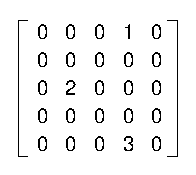
\includegraphics{illustrations/sparse}}
%\afterfig

La representación de la lista contiene un montón de ceros:
\begin{verbatim}
>>> matriz = [ [0,0,0,1,0],
           [0,0,0,0,0],
           [0,2,0,0,0],
           [0,0,0,0,0],
           [0,0,0,3,0] ]
\end{verbatim}

Una posible alternativa consiste en usar un diccionario. Como claves,
podemos usar tuplas que contengan los números de fila y columna. Ésta
es la representación de la misma matriz por medio de un diccionario:
\begin{verbatim}
>>> matriz = {(0,3): 1, (2, 1): 2, (4, 3): 3}
\end{verbatim}

Sólo hay tres pares clave-valor, uno para cada elemento de la matriz
diferente de cero. Cada clave es una tupla, y cada valor es un entero.

Para acceder a un elemento de la matriz, podemos usar el operador
\texttt{{[}{]}}:
\begin{verbatim}
>>> matriz[0,3]
1
\end{verbatim}

Observe que la sintaxis para la representación por medio del diccionario
no es la misma de la representación por medio de la lista anidada.
En lugar de dos índices enteros, usamos un índice compuesto que es
una tupla de enteros.

Hay un problema. Si apuntamos a un elemento que es cero, se produce
un error porque en el diccionario no hay una entrada con esa clave:

\index{error en tiempo de ejecución}
\begin{verbatim}
>>> matriz[1,3]
KeyError: (1, 3)
\end{verbatim}

El método \texttt{get} soluciona este problema:
\begin{verbatim}
>>> matriz.get((0,3), 0)
1
\end{verbatim}

El primer argumento es la clave; el segundo argumento es el valor
que debe devolver \texttt{get} en caso de que la clave no esté en
el diccionario:
\begin{verbatim}
>>> matriz.get((1,3), 0)
0
\end{verbatim}

\texttt{get} mejora sensiblemente la semántica del acceso a una matriz
dispersa. ¡Lástima que la sintaxis no sea tan clara!

\section{Pistas}

\index{pista} \index{función de Fibonacci}

Si ha jugado con la función \texttt{fibonacci} de la Sección~\ref{one more example},
es posible que haya notado que cuanto más grande es el argumento que
recibe, más tiempo le cuesta ejecutarse. De hecho, el tiempo de ejecución
aumenta muy rápidamente. En nuestra máquina, \texttt{fibonacci(20)}
acaba instantáneamente, \texttt{fibonacci(30)} tarda más o menos un
segundo, y \texttt{fibonacci(40)} tarda una eternidad.

Para entender por qué, observe este \textbf{gráfico de llamadas} de
\texttt{fibonacci} con \texttt{n=4}:

\beforefig \centerline{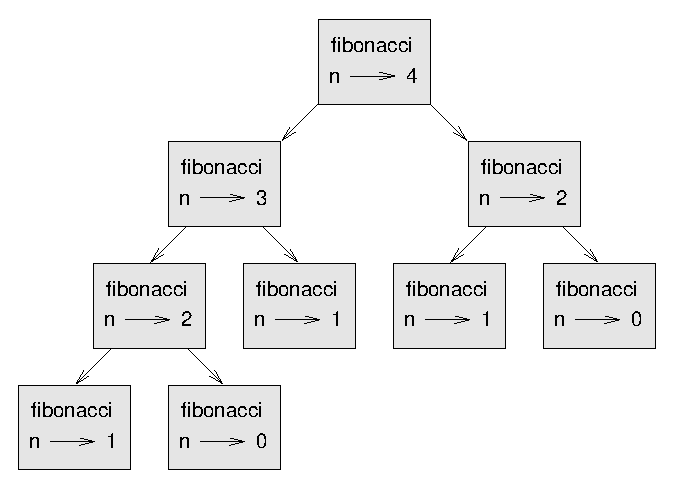
\includegraphics{illustrations/fibonacci}}
\afterfig

Un gráfico de llamadas muestra un conjunto de cajas de función con
líneas que conectan cada caja con las cajas de las funciones a las
que llama. En lo alto del gráfico, \texttt{fibonacci} con \texttt{n=4}
llama a \texttt{fibonacci} con \texttt{n=3} y \texttt{n=2}. A su vez,
\texttt{fibonacci} con \texttt{n=3} llama a \texttt{fibonacci} con
\texttt{n=2} y \texttt{n=1}. Y así sucesivamente.

\index{caja de función} \index{caja} \index{gráfico de llamadas}

Cuente cuántas veces se llama a \texttt{fibonacci(0)} y \texttt{fibonacci(1)}.
Esta función es una solución ineficiente para el problema, y empeora
mucho a medida que crece el argumento.

Una buena solución es llevar un registro de los valores que ya se
han calculado almacenándolos en un diccionario. A un valor que ya
ha sido calculado y almacenado para un uso posterior se le llama \textbf{pista}.
Aquí hay una implementación de \texttt{fibonacci} con pistas:
\begin{verbatim}
anteriores = {0:1, 1:1}

def fibonacci(n):
  if anteriores.has_key(n):
    return anteriores[n]
  else:
    nuevoValor = fibonacci(n-1) + fibonacci(n-2)
    anteriores[n] = nuevoValor
    return nuevoValor
\end{verbatim}

El diccionario llamado \texttt{anteriores} mantiene un registro de
los valores de Fibonacci que ya conocemos. El programa comienza con
sólo dos pares: 0 corresponde a 1 y 1 corresponde a 1.

Siempre que se llama a \texttt{fibonacci} comprueba si el diccionario
contiene el resultado ya calculado. Si está ahí, la función puede
devolver el valor inmediatamente sin hacer más llamadas recursivas.
Si no, tiene que calcular el nuevo valor. El nuevo valor se añade
al diccionario antes de que la función retorne.

Con esta versión de \texttt{fibonacci}, nuestra máquina puede calcular
\texttt{fibonacci(40)} en un abrir y cerrar de ojos. Pero cuando intentamos
calcular \texttt{fibonacci(50)}, nos encontramos con otro problema:

\index{error en tiempo de ejecución} \index{desbordamiento}

\begin{verbatim}
>>> fibonacci(50)
OverflowError: integer addition
\end{verbatim}

La respuesta, como se verá en un momento, es 20.365.011.074. El problema
es que este número es demasiado grande para caber en un entero de
Python. Se \textbf{desborda}. Afortunadamente, hay una solución fácil
para este problema.

\section{Enteros largos}

\index{enteros largos} \index{tipos de datos!enteros largos} \index{enteros!largos}

Python proporciona un tipo llamado \texttt{long int} que puede manejar
enteros de cualquier tamaño. Hay dos formas de crear un valor \texttt{long
int}. Una es escribir un entero con una {\em L} mayúscula al final:

\begin{verbatim}
>>> type(1L)
<type 'long int'>
\end{verbatim}
 La otra es usar la función \texttt{long} para convertir un valor
en \texttt{long int}. \texttt{long} acepta cualquier tipo numérico
e incluso cadenas de dígitos:
\begin{verbatim}
>>> long(1)
1L
>>> long(3.9)
3L
>>> long('57')
57L
\end{verbatim}

Todas las operaciones matemáticas funcionan sobre los datos de tipo
\texttt{long int}, así que no tenemos que hacer mucho para adaptar
\texttt{fibonacci}:
\begin{verbatim}
>>> anteriores = {0:1L, 1:1L}
>>> fibonacci(50)
20365011074L
\end{verbatim}

Simplemente cambiando el contenido inicial de \texttt{anteriores}
cambiamos el comportamiento de \texttt{fibonacci}. Los primeros dos
números de la secuencia son de tipo \texttt{long int}, así que todos
los números subsiguientes lo serán también.

\index{forzado de tipo de datos} \index{coerción!tipo}

\section{Contar letras}

\index{recuento} \index{histograma} \index{compresión}

En el capítulo~\ref{strings} escribimos una función que contaba
el número de apariciones de una letra en una cadena. Una versión más
genérica de este problema es crear un histograma de las letras de
la cadena, o sea, cuántas veces aparece cada letra.

Ese histograma podría ser útil para comprimir un archivo de texto.
Como las diferentes letras aparecen con frecuencias distintas, podemos
comprimir un archivo usando códigos cortos para las letras más habituales
y códigos más largos para las que aparecen con menor frecuencia.

Los diccionarios facilitan una forma elegante de generar un histograma:
\begin{verbatim}
>>> cuentaLetras = {}
>>> for letra in "Mississippi":
      cuentaLetras[letra] = cuentaLetras.get(letra, 0)+1

>>> cuentaLetras
{'M': 1, 's': 4, 'p': 2, 'i': 4}
\end{verbatim}

Inicialmente, tenemos un diccionario vacío. Para cada letra de la
cadena, buscamos el recuento actual (posiblemente cero) y la incrementamos.
Al final, el diccionario contiene pares de letras y sus frecuencias.

Puede ser más atractivo mostrar el histograma en orden alfabético.
Podemos hacerlo con los métodos \texttt{items} y \texttt{sort}:
\begin{verbatim}
>>> itemsLetras = cuentaLetras.items()
>>> list(itemsLetras).sort()
>>> print(itemsLetras)
[('M', 1), ('i', 4), ('p', 2), ('s', 4)]
\end{verbatim}

Usted ya ha visto el método \texttt{items} aplicable a los diccionarios;
\texttt{sort} es un método aplicable a listas. Hay varios más, como
\texttt{append}, \texttt{extend} y \texttt{reverse}. Consulte la documentación
de Python para ver los detalles.

\index{método!lista} \index{método de lista}

\section{Glosario}
\begin{description}
\item [{Diccionario:}] es una colección de pares clave-valor que establece
una correspondencia entre claves y valores. Las claves pueden ser
de cualquier tipo inmutable, los valores pueden ser de cualquier tipo.
\item [{Clave:}] un valor que se usa para buscar una entrada en un diccionario.
\item [{Par clave-valor:}] uno de los elementos de un diccionario, también
llamado ``asociación''.
\item [{Método:}] tipo de función al que se llama con una sintaxis diferente
y al que se invoca ``sobre'' un objeto.
\item [{Invocar:}] llamar a un método.
\item [{Pista:}] almacenamiento temporal de un valor precalculado, para
evitar cálculos redundantes.
\item [{Desbordamiento:}] resultado numérico que es demasiado grande para
representarse en formato numérico.

\index{diccionario} \index{clave} \index{par clave-valor} \index{pista}
\index{método} \index{invocar}
\end{description}

\section{Ejercicios}

Para cada función, agregue chequeo de tipos y pruebas unitarias.
\begin{enumerate}
\item Como ejercicio, modifique \texttt{factorial} de forma que produzca
un \texttt{long int} como resultado.
\item Escriba una función booleana que averigüe si una lista tiene algún
elemento duplicado usando un diccionario.
\item Una cadena de ARN puede representarse como una lista en la que los
elementos pueden ser los caracteres A,C,G y U. Escriba una función
booleana que averigüe si una lista de caracteres es una cadena de
ARN válida.
\item Generalice la función anterior de forma que reciba una biosecuencia
(ADN, ARN ó Proteína) y un alfabeto de referencia para averiguar si
está bien formada. Para ADN el alfabeto es A,C,T y G, para las proteínas
es:

A,R,N,D,C,E,Q,G,H,I,L,K,M,F,P,S,T,W,Y,V,U,O
\item Escriba una función que reciba una cadena de ADN y cuente cuantos
nucleótidos de cada tipo tiene (cuantas veces tiene A,C,G y T) usando
un diccionario.
\item Generalice la función anterior de forma que reciba una biosecuencia
(ADN, ARN ó Proteína) y un alfabeto. Debe contar cuantos elementos
tiene de cada tipo usando un diccionario.
\item Escriba una función producto que reciba una matriz dispersa M, implementada
con un diccionario, y un número. Debe retornar la matriz que resulta
de multiplicar cada elemento de M por el número.
\item Escriba una función que reciba dos matrices dispersas, implementadas
con diccionarios, y las sume, produciendo otra matriz dispersa.
\item Escriba una función que reciba dos matrices dispersas, implementadas
con diccionarios, y las multiplique, produciendo otra matriz dispersa.
Base su solución en las dos soluciones anteriores.
\item Escriba una función booleana que reciba una matriz dispersa y averigüe
si es la matriz identidad. 
\end{enumerate}

